% Chiplet Studio internal architecture: UI over Engine over external deps.
\documentclass[border=3mm]{standalone}
\usepackage{tikz}
\usetikzlibrary{arrows.meta, positioning, calc, fit, backgrounds}
\usepackage[T1]{fontenc}
\usepackage{lmodern}

\definecolor{IHPfg}{RGB}{0,80,139}
\definecolor{IHPaccent}{RGB}{109,112,114}
\definecolor{IHPlight}{RGB}{225,238,250}
\definecolor{cUI}{RGB}{55,145,195}
\definecolor{cEngine}{RGB}{0,80,139}
\definecolor{cExt}{RGB}{72,75,77}

\begin{document}
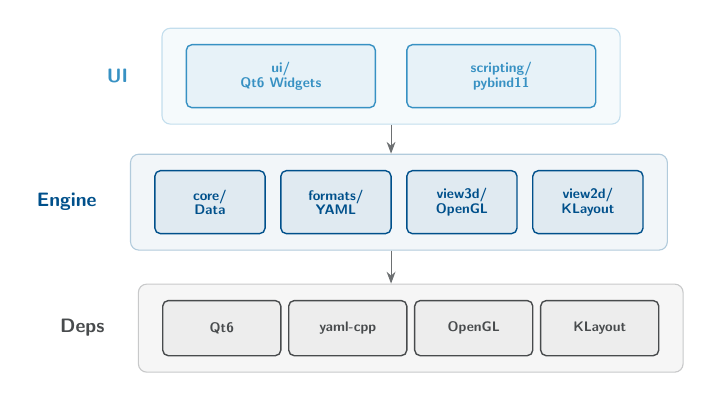
\begin{tikzpicture}[
    >=Stealth,
    modbox/.style={
        rectangle, rounded corners=2pt,
        draw=#1, fill=#1!12, line width=0.5pt,
        minimum height=8mm,
        font=\sffamily\tiny\bfseries, text=#1, align=center
    },
    layerlbl/.style={
        font=\sffamily\scriptsize\bfseries, text=#1, anchor=east
    },
    extbox/.style={
        rectangle, rounded corners=2pt,
        draw=cExt, fill=cExt!10, line width=0.5pt,
        minimum width=15mm, minimum height=7mm,
        font=\sffamily\tiny\bfseries, text=cExt, align=center
    },
    layerbg/.style={
        rectangle, rounded corners=3pt,
        fill=#1!5, draw=#1!30, line width=0.4pt
    }
]

% ======== Layer 1: UI (top) ========
\node[modbox=cUI, minimum width=24mm] (ui) at (0, 0) {ui/\\[-0.3mm]Qt6 Widgets};
\node[modbox=cUI, minimum width=24mm] (script) at (2.8, 0) {scripting/\\[-0.3mm]pybind11};

\begin{scope}[on background layer]
    \node[layerbg=cUI, fit=(ui)(script), inner xsep=3mm, inner ysep=2mm] (uilayer) {};
\end{scope}
\node[layerlbl=cUI] at ([xshift=-3mm]uilayer.west) {UI};

% ======== Layer 2: Engine (middle) ========
\node[modbox=cEngine, minimum width=14mm] (core) at (-0.9, -1.6) {core/\\[-0.3mm]Data};
\node[modbox=cEngine, minimum width=14mm] (fmt) at (0.7, -1.6) {formats/\\[-0.3mm]YAML};
\node[modbox=cEngine, minimum width=14mm] (v3d) at (2.3, -1.6) {view3d/\\[-0.3mm]OpenGL};
\node[modbox=cEngine, minimum width=14mm] (v2d) at (3.9, -1.6) {view2d/\\[-0.3mm]KLayout};

\begin{scope}[on background layer]
    \node[layerbg=cEngine, fit=(core)(fmt)(v3d)(v2d), inner xsep=3mm, inner ysep=2mm] (englayer) {};
\end{scope}
\node[layerlbl=cEngine] at ([xshift=-3mm]englayer.west) {Engine};

% ======== Layer 3: External deps (bottom) ========
\node[extbox] (qt6) at (-0.75, -3.2) {Qt6};
\node[extbox] (ycpp) at (0.85, -3.2) {yaml-cpp};
\node[extbox] (ogl) at (2.45, -3.2) {OpenGL};
\node[extbox] (kl) at (4.05, -3.2) {KLayout};

\begin{scope}[on background layer]
    \node[layerbg=cExt, fit=(qt6)(ycpp)(ogl)(kl), inner xsep=3mm, inner ysep=2mm] (extlayer) {};
\end{scope}
\node[layerlbl=cExt] at ([xshift=-3mm]extlayer.west) {Deps};

% ======== Arrows between layers (perfectly vertical at x=1.4) ========
\draw[-{Stealth[length=1.5mm]}, line width=0.4pt, color=IHPaccent]
    (uilayer.south -| 1.4,0) -- (englayer.north -| 1.4,0);
\draw[-{Stealth[length=1.5mm]}, line width=0.4pt, color=IHPaccent]
    (englayer.south -| 1.4,0) -- (extlayer.north -| 1.4,0);

\end{tikzpicture}
\end{document}
